%%% Math 340
%%% Homework 3

\documentclass{article}

\usepackage[utf8]{inputenc}
\usepackage[top=1.5in,left=1in,right=1in,bottom=1.5in,headheight=1in]{geometry}
\usepackage{fancyhdr}
\usepackage{lastpage}
\usepackage{amsmath,amsthm}
\usepackage{enumerate}
\usepackage{tikz}
\usepackage{multicol}
\usepackage{graphicx}

\newtheoremstyle{problem}
{1cm}% Above space
{1cm}% Below space
{}%         Body font
{}%         Indent amount (empty = no indent, \parindent = para indent)
{\bfseries}% Thm head font
{\vspace{5pt}}%        Punctuation after thm head
{\newline}%     Space after thm head (\newline = linebreak)
{\thmname{#1}\thmnote{ #3}\\}%         Thm head spec

\theoremstyle{problem}
\newtheorem{prob}{Problem}

%%% Heading -- No need to edit %%%
\pagestyle{fancy}
\rhead{
  Stefan Eng \\ 
  William Watkins \\ 
  Math 340 \\ 
  9/23/13
}
\lhead{
  Chapter 3\\
  1, 3, 9, 23, 27, 35, 41
}
\cfoot{Page\ \thepage\ of\ \pageref{LastPage}}
%%% 

% No indent for whole page
\setlength\parindent{0pt}

\def\Acircle{(180:1cm) circle (2cm)}
\def\Bcircle{(0:1cm) circle (2cm)}
\def\ABComp{(-3.5,-2.5) rectangle (3.5,2.5)}

\begin{document}

%%% Make the title %%%
\begin{center}
  \textsc{\Large Introduction to Probability}\\[.3cm]
  \textsc{\Large Homework 4}
\end{center}
%%% End title %%%

%%% Start Assignment Here %%%
\begin{prob}[1]
 
\end{prob}
\begin{multicols}{2}
  Given that $20\%$ of wells had no impurities, \\$40\%$ has impurity A and $50\%$ had impurity B \\
 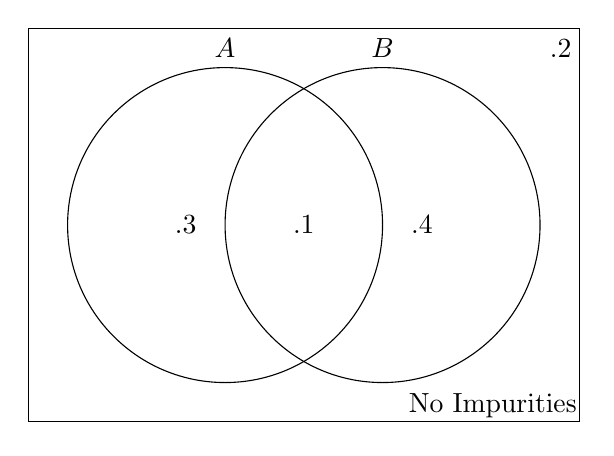
\begin{tikzpicture}
    \begin{scope}
      \draw \ABComp ++(-.5,-.5)node[text=black,above right] {$.2$} (2.4,-2.3)node[text=black] {No Impurities};
      \draw \Acircle ++(0,2)node[text=black,above] {$A$} ++(-.5,-2)node[text=black] {$.3$};
      \draw \Bcircle ++(0,2)node[text=black,above] {$B$} ++(.5,-2)node[text=black] {$.4$};
      \draw (0,0) node [text=black] {$.1$};
    \end{scope}
  \end{tikzpicture}
  \vfill
  \columnbreak
  We can see from our Venn Diagram that, $$P(A \cup B) = .8$$ So, by the Additive Law, 
  \begin{align*}
    P(A \cup B) &= P(A) + P(B) - P(A \cap B)\\
    P(A \cap B) &= P(A) + P(B) - P(A \cup B)\\
                &= .4 + .5 - .8\\
                &= .1
  \end{align*}
    Thus, $P(A \cap B) = .1$.\\[.5cm]
 
  \begin{tabular}{r|c c c}
    & 0 & 1 & 2 \\
    \hline
    p(y) & .2 & .7 & .1
  \end{tabular}
\end{multicols}

\begin{prob}[3]
\begin{multicols}{2}

\begin{tabular}{r|c c c c}
Device & 1 & 2 & 3 & 4\\
\hline
p(y) & 0 & $\frac{1}{6}$ & $\frac{2}{6}$ & $\frac{3}{6}$\\
\end{tabular}
\vfill
\columnbreak
  There are ${4 \choose 2} = 6$ ways to pick the components. The probability distribution Y, the number of the test on which the second defective device is found, is as shown on the left.
\end{multicols}
\end{prob}

\begin{prob}[9]
Assume that the company's employees make erroneous entries $5\%$ of the time.
    \begin{figure}
      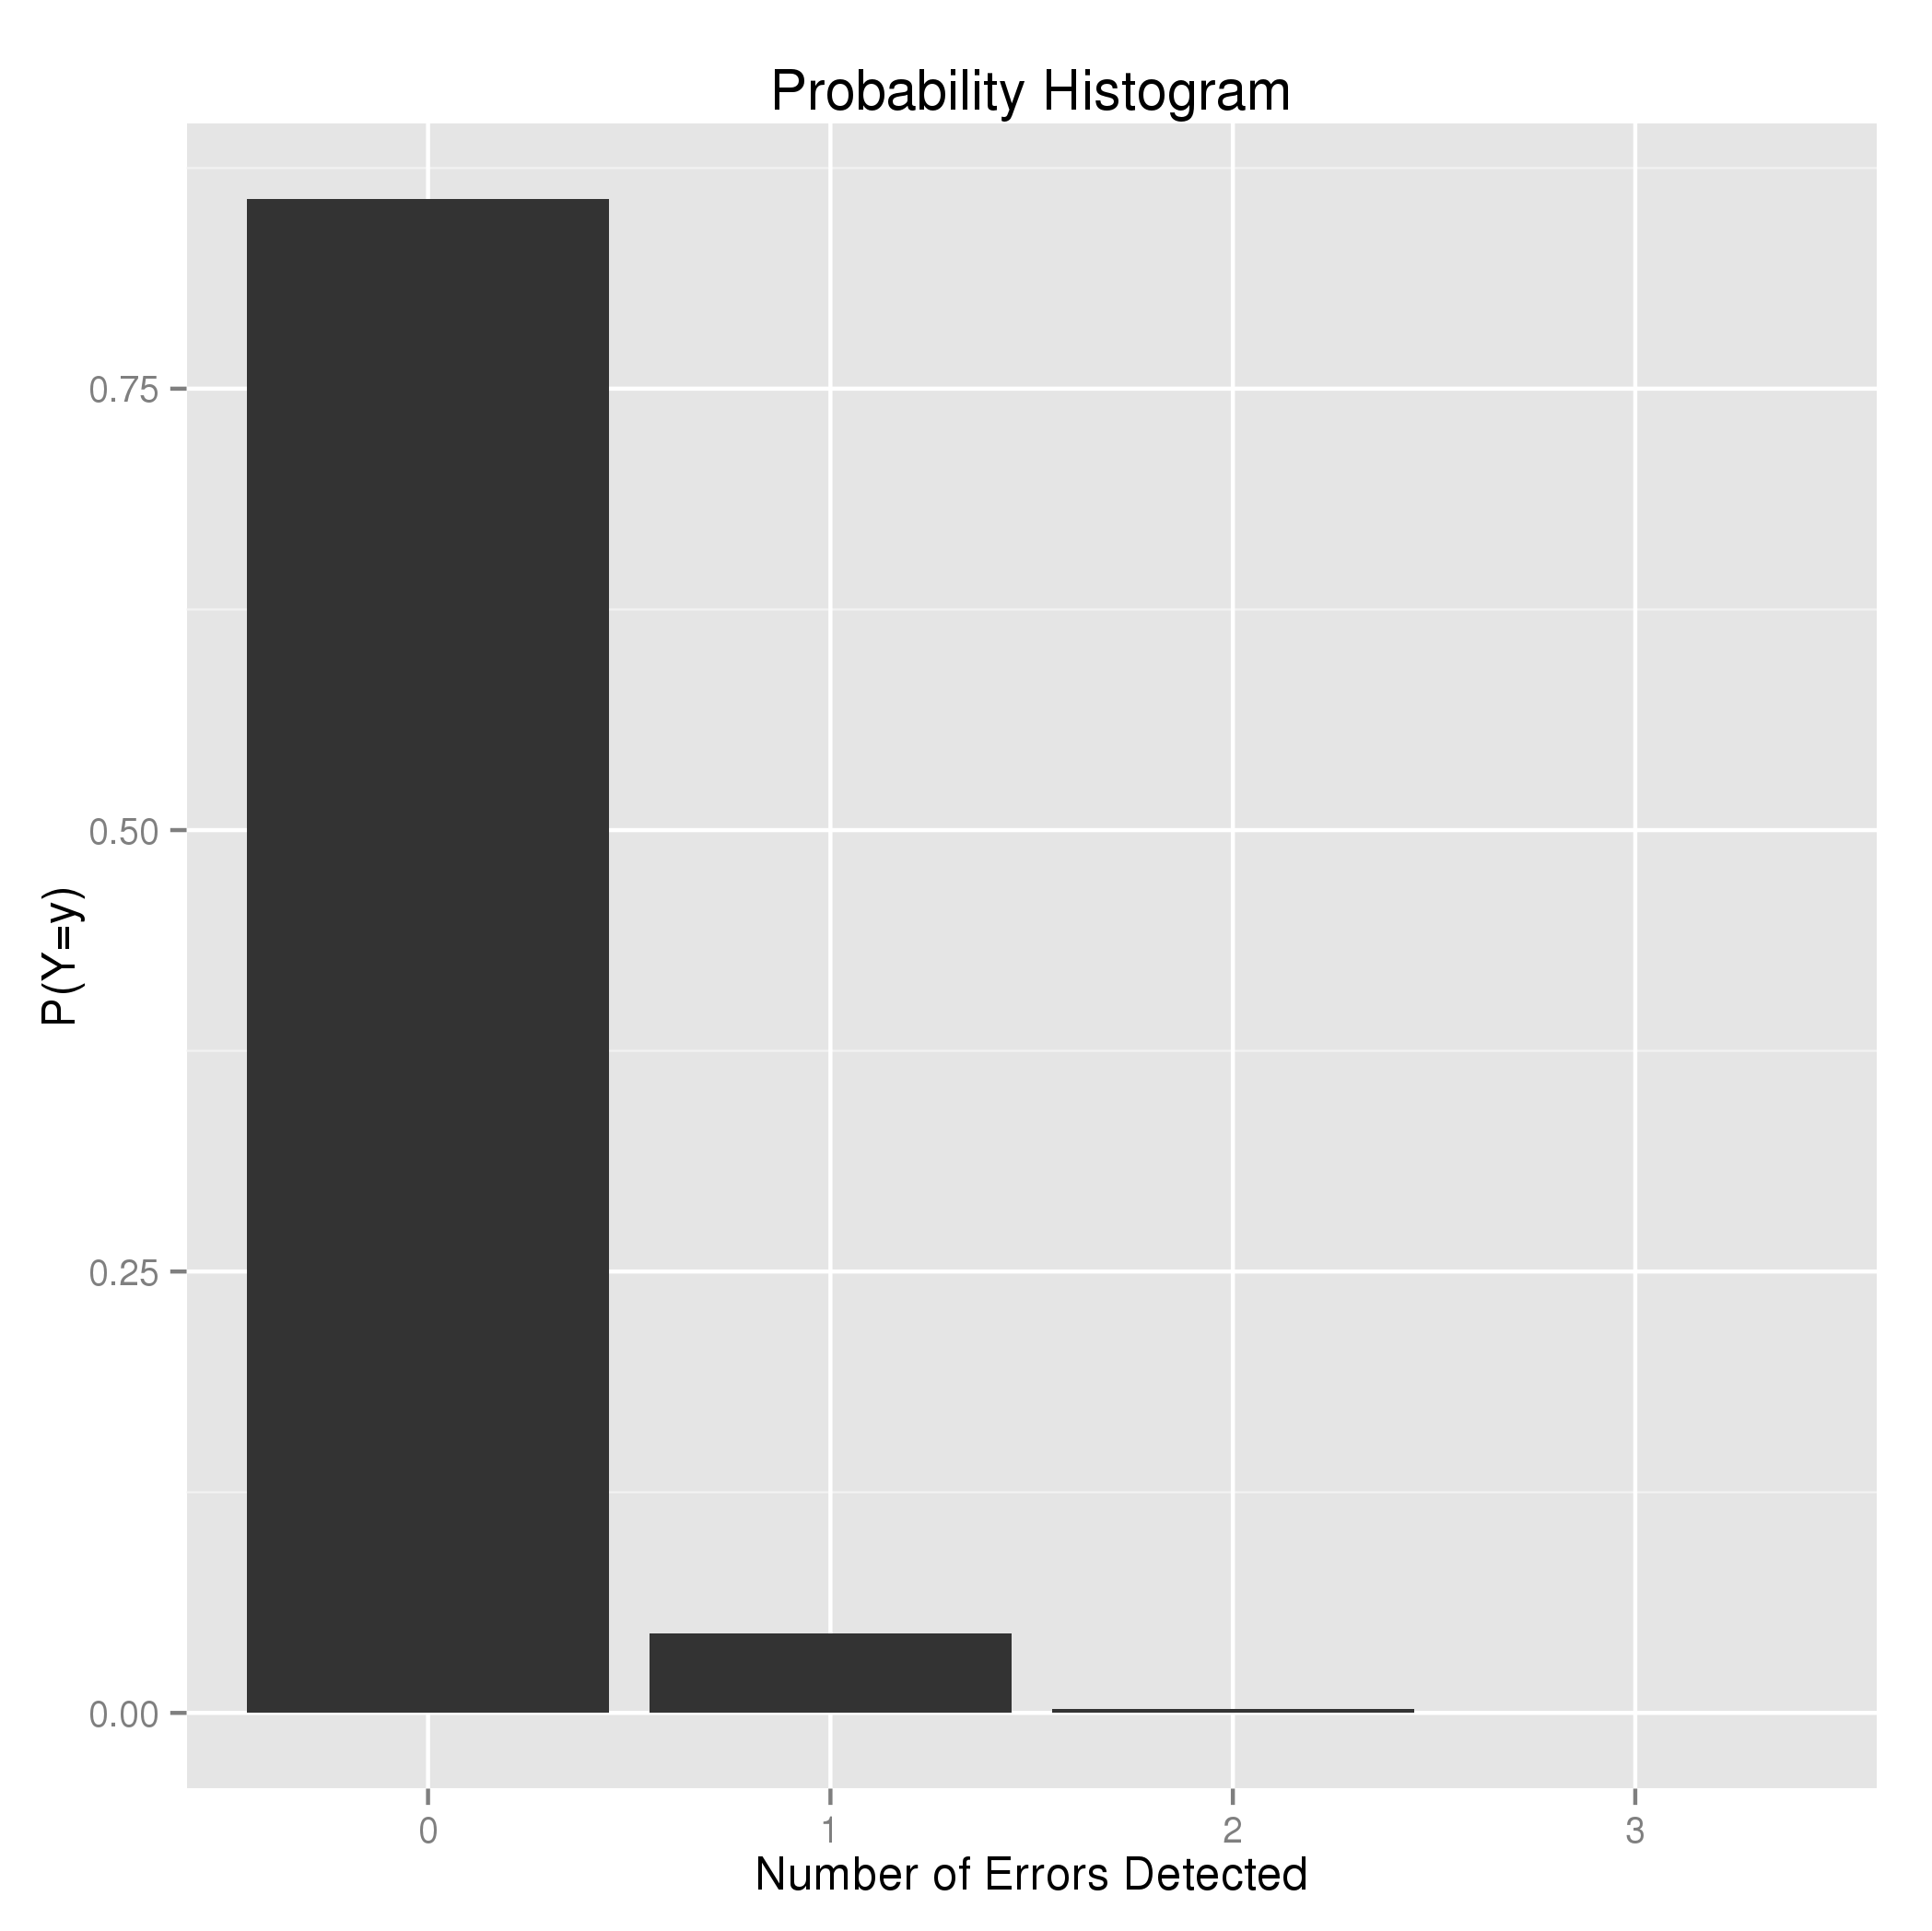
\includegraphics{hist_prob9.png}
    \end{figure}
\end{prob}

\begin{prob}[23]
  
\end{prob}
\end{document}

%%% End assignment %%%
